% Created by tikzDevice version 0.12.3.1 on 2021-05-04 17:12:41
% !TEX encoding = UTF-8 Unicode
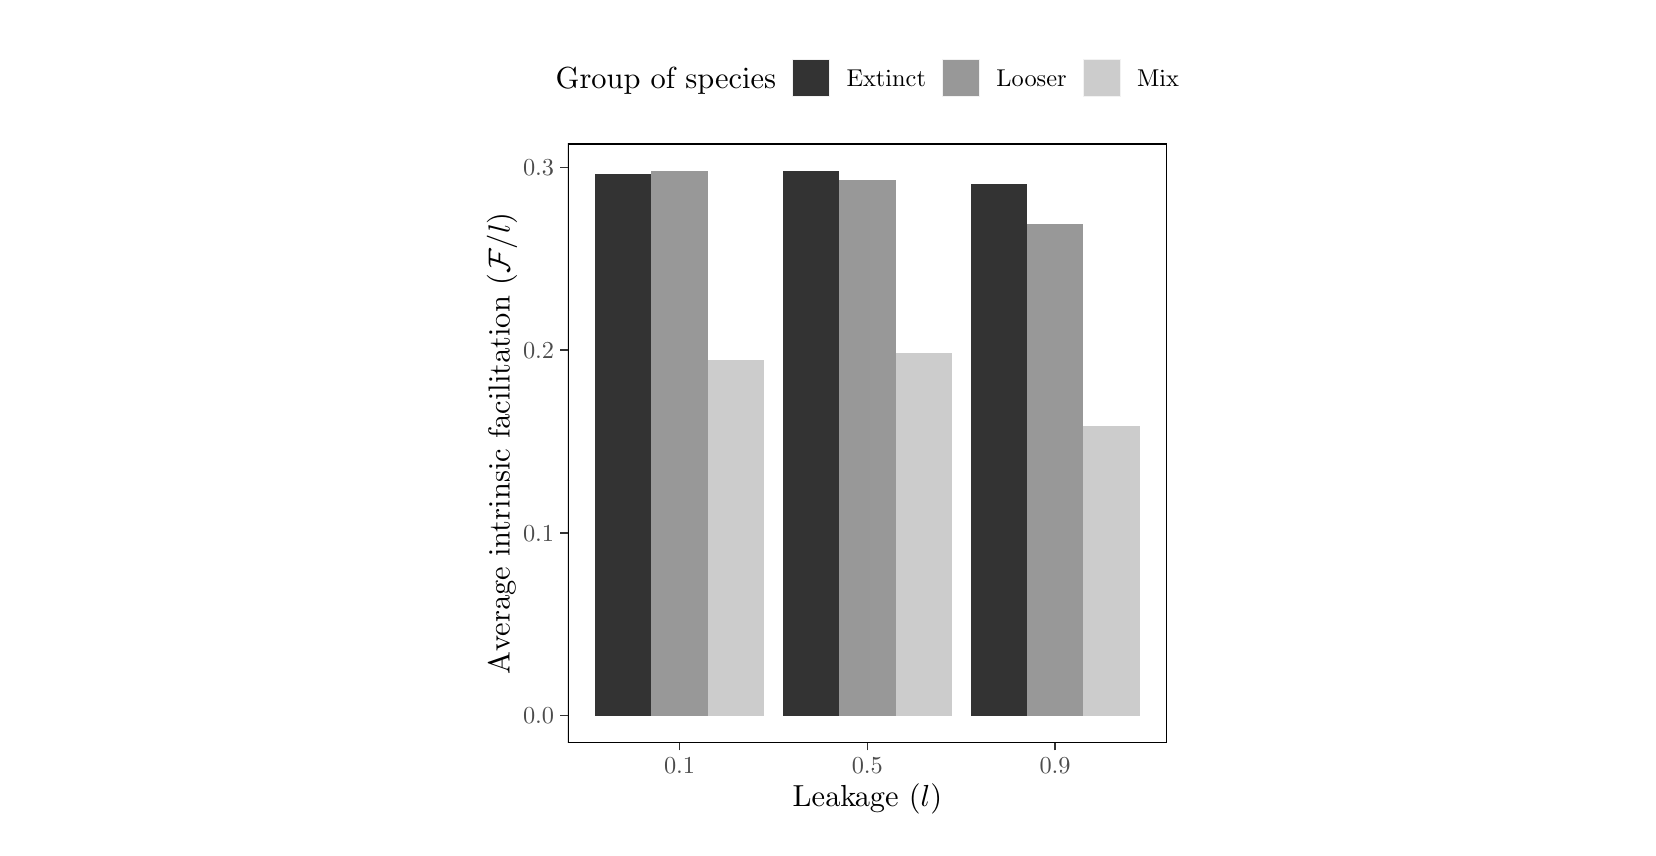
\begin{tikzpicture}[x=1pt,y=1pt]
\definecolor{fillColor}{RGB}{255,255,255}
\path[use as bounding box,fill=fillColor,fill opacity=0.00] (0,0) rectangle (578.16,289.08);
\begin{scope}
\path[clip] (161.03,  0.00) rectangle (417.13,289.08);
\definecolor{drawColor}{RGB}{255,255,255}
\definecolor{fillColor}{RGB}{255,255,255}

\path[draw=drawColor,line width= 0.6pt,line join=round,line cap=round,fill=fillColor] (161.03,  0.00) rectangle (417.13,289.08);
\end{scope}
\begin{scope}
\path[clip] (195.19, 30.69) rectangle (411.63,247.13);

\path[] (195.19, 30.69) rectangle (411.63,247.13);
\definecolor{drawColor}{RGB}{255,255,255}

\path[draw=drawColor,line width= 0.3pt,line join=round] (195.19, 73.53) --
	(411.63, 73.53);

\path[draw=drawColor,line width= 0.3pt,line join=round] (195.19,139.54) --
	(411.63,139.54);

\path[draw=drawColor,line width= 0.3pt,line join=round] (195.19,205.55) --
	(411.63,205.55);

\path[draw=drawColor,line width= 0.3pt,line join=round] (201.63, 30.69) --
	(201.63,247.13);

\path[draw=drawColor,line width= 0.3pt,line join=round] (269.48, 30.69) --
	(269.48,247.13);

\path[draw=drawColor,line width= 0.3pt,line join=round] (337.33, 30.69) --
	(337.33,247.13);

\path[draw=drawColor,line width= 0.3pt,line join=round] (405.18, 30.69) --
	(405.18,247.13);

\path[draw=drawColor,line width= 0.6pt,line join=round] (195.19, 40.52) --
	(411.63, 40.52);

\path[draw=drawColor,line width= 0.6pt,line join=round] (195.19,106.53) --
	(411.63,106.53);

\path[draw=drawColor,line width= 0.6pt,line join=round] (195.19,172.55) --
	(411.63,172.55);

\path[draw=drawColor,line width= 0.6pt,line join=round] (195.19,238.56) --
	(411.63,238.56);

\path[draw=drawColor,line width= 0.6pt,line join=round] (235.56, 30.69) --
	(235.56,247.13);

\path[draw=drawColor,line width= 0.6pt,line join=round] (303.41, 30.69) --
	(303.41,247.13);

\path[draw=drawColor,line width= 0.6pt,line join=round] (371.26, 30.69) --
	(371.26,247.13);
\definecolor{fillColor}{gray}{0.80}

\path[fill=fillColor] (245.74, 40.52) rectangle (266.09,168.87);
\definecolor{fillColor}{RGB}{152,152,152}

\path[fill=fillColor] (225.38, 40.52) rectangle (245.74,237.15);
\definecolor{fillColor}{gray}{0.20}

\path[fill=fillColor] (205.03, 40.52) rectangle (225.38,236.31);
\definecolor{fillColor}{gray}{0.80}

\path[fill=fillColor] (313.59, 40.52) rectangle (333.94,171.37);
\definecolor{fillColor}{RGB}{152,152,152}

\path[fill=fillColor] (293.23, 40.52) rectangle (313.59,234.09);
\definecolor{fillColor}{gray}{0.20}

\path[fill=fillColor] (272.88, 40.52) rectangle (293.23,237.29);
\definecolor{fillColor}{gray}{0.80}

\path[fill=fillColor] (381.44, 40.52) rectangle (401.79,145.05);
\definecolor{fillColor}{RGB}{152,152,152}

\path[fill=fillColor] (361.08, 40.52) rectangle (381.44,218.31);
\definecolor{fillColor}{gray}{0.20}

\path[fill=fillColor] (340.73, 40.52) rectangle (361.08,232.48);
\definecolor{drawColor}{RGB}{0,0,0}

\path[draw=drawColor,line width= 0.6pt,line join=round,line cap=round] (195.19, 30.69) rectangle (411.63,247.13);
\end{scope}
\begin{scope}
\path[clip] (  0.00,  0.00) rectangle (578.16,289.08);
\definecolor{drawColor}{gray}{0.30}

\node[text=drawColor,anchor=base east,inner sep=0pt, outer sep=0pt, scale=  0.88] at (190.24, 37.49) {0.0};

\node[text=drawColor,anchor=base east,inner sep=0pt, outer sep=0pt, scale=  0.88] at (190.24,103.50) {0.1};

\node[text=drawColor,anchor=base east,inner sep=0pt, outer sep=0pt, scale=  0.88] at (190.24,169.52) {0.2};

\node[text=drawColor,anchor=base east,inner sep=0pt, outer sep=0pt, scale=  0.88] at (190.24,235.53) {0.3};
\end{scope}
\begin{scope}
\path[clip] (  0.00,  0.00) rectangle (578.16,289.08);
\definecolor{drawColor}{gray}{0.20}

\path[draw=drawColor,line width= 0.6pt,line join=round] (192.44, 40.52) --
	(195.19, 40.52);

\path[draw=drawColor,line width= 0.6pt,line join=round] (192.44,106.53) --
	(195.19,106.53);

\path[draw=drawColor,line width= 0.6pt,line join=round] (192.44,172.55) --
	(195.19,172.55);

\path[draw=drawColor,line width= 0.6pt,line join=round] (192.44,238.56) --
	(195.19,238.56);
\end{scope}
\begin{scope}
\path[clip] (  0.00,  0.00) rectangle (578.16,289.08);
\definecolor{drawColor}{gray}{0.20}

\path[draw=drawColor,line width= 0.6pt,line join=round] (235.56, 27.94) --
	(235.56, 30.69);

\path[draw=drawColor,line width= 0.6pt,line join=round] (303.41, 27.94) --
	(303.41, 30.69);

\path[draw=drawColor,line width= 0.6pt,line join=round] (371.26, 27.94) --
	(371.26, 30.69);
\end{scope}
\begin{scope}
\path[clip] (  0.00,  0.00) rectangle (578.16,289.08);
\definecolor{drawColor}{gray}{0.30}

\node[text=drawColor,anchor=base,inner sep=0pt, outer sep=0pt, scale=  0.88] at (235.56, 19.68) {0.1};

\node[text=drawColor,anchor=base,inner sep=0pt, outer sep=0pt, scale=  0.88] at (303.41, 19.68) {0.5};

\node[text=drawColor,anchor=base,inner sep=0pt, outer sep=0pt, scale=  0.88] at (371.26, 19.68) {0.9};
\end{scope}
\begin{scope}
\path[clip] (  0.00,  0.00) rectangle (578.16,289.08);
\definecolor{drawColor}{RGB}{0,0,0}

\node[text=drawColor,anchor=base,inner sep=0pt, outer sep=0pt, scale=  1.10] at (303.41,  7.64) {Leakage $(l)$};
\end{scope}
\begin{scope}
\path[clip] (  0.00,  0.00) rectangle (578.16,289.08);
\definecolor{drawColor}{RGB}{0,0,0}

\node[text=drawColor,rotate= 90.00,anchor=base,inner sep=0pt, outer sep=0pt, scale=  1.10] at (174.11,138.91) {Average intrinsic facilitation ($\mathcal{F}/l$)};
\end{scope}
\begin{scope}
\path[clip] (  0.00,  0.00) rectangle (578.16,289.08);
\definecolor{fillColor}{RGB}{255,255,255}

\path[fill=fillColor] (185.28,258.13) rectangle (421.53,283.58);
\end{scope}
\begin{scope}
\path[clip] (  0.00,  0.00) rectangle (578.16,289.08);
\definecolor{drawColor}{RGB}{0,0,0}

\node[text=drawColor,anchor=base west,inner sep=0pt, outer sep=0pt, scale=  1.10] at (190.78,267.07) {Group of species};
\end{scope}
\begin{scope}
\path[clip] (  0.00,  0.00) rectangle (578.16,289.08);
\definecolor{drawColor}{RGB}{255,255,255}
\definecolor{fillColor}{gray}{0.95}

\path[draw=drawColor,line width= 0.6pt,line join=round,line cap=round,fill=fillColor] (275.94,263.63) rectangle (290.39,278.08);
\end{scope}
\begin{scope}
\path[clip] (  0.00,  0.00) rectangle (578.16,289.08);
\definecolor{fillColor}{gray}{0.20}

\path[fill=fillColor] (276.65,264.34) rectangle (289.68,277.37);
\end{scope}
\begin{scope}
\path[clip] (  0.00,  0.00) rectangle (578.16,289.08);
\definecolor{drawColor}{RGB}{255,255,255}
\definecolor{fillColor}{gray}{0.95}

\path[draw=drawColor,line width= 0.6pt,line join=round,line cap=round,fill=fillColor] (330.11,263.63) rectangle (344.56,278.08);
\end{scope}
\begin{scope}
\path[clip] (  0.00,  0.00) rectangle (578.16,289.08);
\definecolor{fillColor}{RGB}{152,152,152}

\path[fill=fillColor] (330.82,264.34) rectangle (343.85,277.37);
\end{scope}
\begin{scope}
\path[clip] (  0.00,  0.00) rectangle (578.16,289.08);
\definecolor{drawColor}{RGB}{255,255,255}
\definecolor{fillColor}{gray}{0.95}

\path[draw=drawColor,line width= 0.6pt,line join=round,line cap=round,fill=fillColor] (380.93,263.63) rectangle (395.38,278.08);
\end{scope}
\begin{scope}
\path[clip] (  0.00,  0.00) rectangle (578.16,289.08);
\definecolor{fillColor}{gray}{0.80}

\path[fill=fillColor] (381.64,264.34) rectangle (394.67,277.37);
\end{scope}
\begin{scope}
\path[clip] (  0.00,  0.00) rectangle (578.16,289.08);
\definecolor{drawColor}{RGB}{0,0,0}

\node[text=drawColor,anchor=base west,inner sep=0pt, outer sep=0pt, scale=  0.88] at (295.89,267.82) {Extinct};
\end{scope}
\begin{scope}
\path[clip] (  0.00,  0.00) rectangle (578.16,289.08);
\definecolor{drawColor}{RGB}{0,0,0}

\node[text=drawColor,anchor=base west,inner sep=0pt, outer sep=0pt, scale=  0.88] at (350.06,267.82) {Looser};
\end{scope}
\begin{scope}
\path[clip] (  0.00,  0.00) rectangle (578.16,289.08);
\definecolor{drawColor}{RGB}{0,0,0}

\node[text=drawColor,anchor=base west,inner sep=0pt, outer sep=0pt, scale=  0.88] at (400.88,267.82) {Mix};
\end{scope}
\end{tikzpicture}
